%%%%%%%%%%%%%%%%%%%%%%%%%%%%%%%%%%%%%%%%%%%%%%%%%%%%%%%%%%%%%%%%%%%%%%%%%%%%%%%%
%2345678901234567890123456789012345678901234567890123456789012345678901234567890
%        1         2         3         4         5         6         7         8
% THESIS Chapter

\chapter{Background}

In this section I will discuss some of the existing approaches to dynamic network visualisation and network measures. I will then provide additional details on measures in this context and The Vistorian's technologies, interface, format and background.

\section{Dynamic Network Visualisation Techniques}

%Whilst this report will focus on using measure visualisations as a dynamic network visualisation technique it can be useful to see other approaches to visualising dynamic networks. 

\subsection{State of the Art}
Beck et al. \cite{tsotaivg} reviewed 129 peer-reviewed publications on dynamic network visualisation from 1992 to 2014.  Three categories of dynamic network visualisation were highlighted: animation, timeline and hybrid. Animations, or time-to-time mappings, display the network at each point in time sequentially - creating an animation. In timelines, or time-to-space mappings, the networks are drawn along this timeline in some manner - there are a variety of ways this can be done as shown in Figure \ref{timeLineApproaches}. 
\begin{figure}[H]
\begin{center}
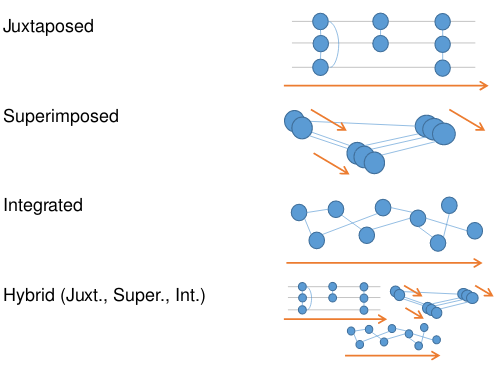
\includegraphics[trim={0 0 0 0}, width=70mm]{./Figures/timeLineApproaches.png}
\caption{
Juxtaposed - networks are simply placed next to each other.\newline
Superimposed - networks are 'stacked' on top of each other.\newline
Integrated - the timeline is woven directly into the graph.\newline
Hybrid - combining the above approaches in some manner.\newline
Figure and descriptions taken from Beck et al. \cite{tsotaivg}.}
\label{timeLineApproaches}
\end{center}
\end{figure}
Two sub-categories to the timeline approach are given: nodelink diagrams and adjacency matrixes, shown in Figure \ref{nlVsAdjMat}. None of the publications reviewed took a measure based approach.


\begin{figure}[H]
\begin{center}
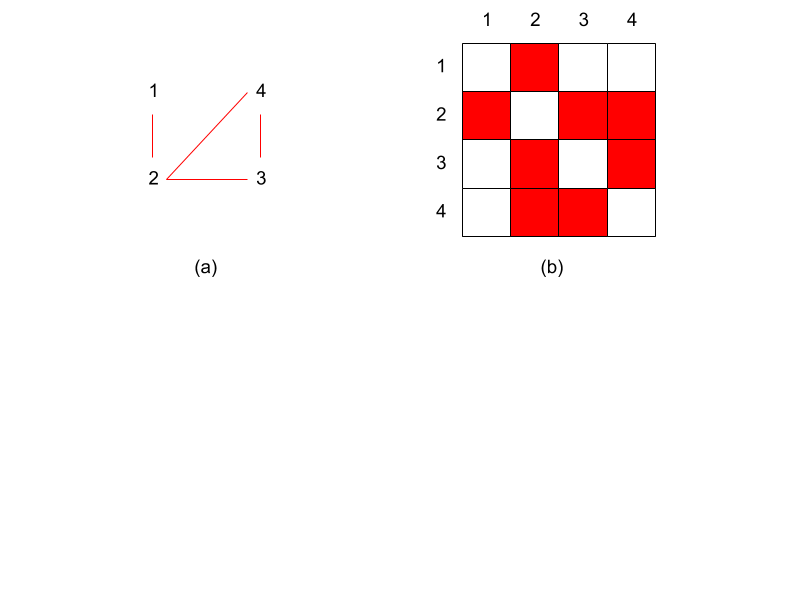
\includegraphics[trim={0 10cm 0 0}, width=140mm]{./Figures/nlVsAdjMat.png}
\caption{Nodelink diagram (a) and it's corresponding Adjacency Matrix (b)}
\label{nlVsAdjMat}
\end{center}
\end{figure}

\subsection{Dynamic Network Visualisation Tools}
\subsubsection*{Sonia}
SoNIA \cite{sonia} is a node-link animation based dynamic network visualisation tool that aims "to handle network data and visualization in ways that explicitly deal with its time-based nature and aids the user in understanding what their data really mean" \cite{taasodnv}. SoNIA can be used to save the network animation as a quicktime movie. An interesting technique used in SoNIA is the interpolation of points between changes, to create smoother transitions that are more easily followed by the human eye. SoNIA has been successfully used for modelling interaction networks, disease transmission and football passing patterns demonstrating that animations are a feasible tool for visualising changes in network structure.

\begin{figure}[H]
\begin{center}
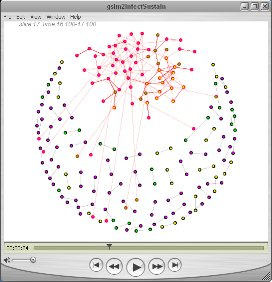
\includegraphics[trim={0 0 0 0}, width=70mm]{./Figures/soniaPic.jpg}
\caption{A SoNIA generated movie - \cite{soniaDiagram}}
\end{center}
\end{figure}

\subsubsection*{Matrix Cubes}
Matrix Cubes \cite{vdnwmc} takes adjacency matrixes and applies the technique to dynamic networks. Matrix cubes use the adjacency matrix of each static slice of a dynamic network and stack them next to each other in order - using time as the third dimension, creating a cube. 

\begin{figure}[H]
\begin{center}
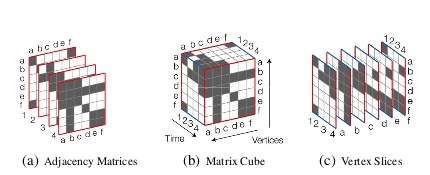
\includegraphics[trim={0 0 0 0}, width=140mm]{./Figures/networkCubePic.png}
\caption{Matrix Cube Structure \cite{vdnwmc}.}
\end{center}
\end{figure}
%Matrixes are more readable for larger and denser graphs with nodelink found to be worse than a matrix representation for static networks composed of over 20 nodes \cite{acotrogunlambr}.

\subsubsection*{GraphCuisine}
Measures have been used to characterise networks. GraphCuisine \cite{gcuisine} is a random graph generator where the generated graph is encoded as a set of weighted measures, such as the number of nodes, density and clustering coefficient. GraphCuisine can only generate static networks. The user interface is shown in Figure \ref{fig:graphCuisineInUse}.


\begin{figure}[H]
  \begin{center}
  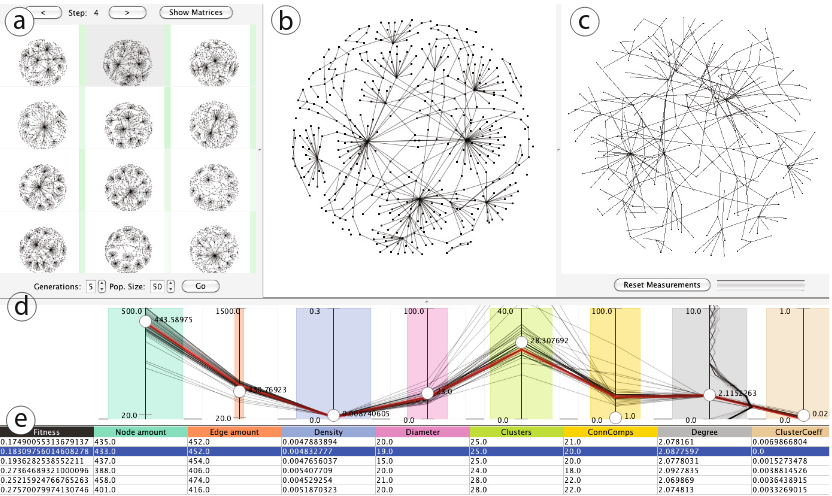
\includegraphics[trim={0 0 0 0}, width=140mm]{./Figures/graphCuisineInUse.png}
  \caption{
    User Interface of GraphCuisine showing (a) the population view, displaying representative graphs of the current population; (b) the detail  view of the selected graph; (c) an imported graph in the dataset view, (d) a parallel coordinates plot in the measurement view showing the distribution of measures in the population, and (e) the measures table with an entry for each representative graphs. In the measures view, the target measures are indicated by the position of the white markers, while black polylines line show the measures of the selected graph.\newline
    Figure and description taken from Interactive Random Graph Generation with Evolutionary Algorithms \cite{gcuisine}. 
    }
  \label{fig:graphCuisineInUse}
  \end{center}
\end{figure}

\subsubsection*{Clustering Associated Temporal Attributes}
Measures have been plotted over time to illustrate temporal trends in a network. Hadlak et al. \cite{dynamicTrend} provide a tool to discover substructures with similar trends. Three similarity measures are provided to select between: Euclidean distance, correlation coefficient and a trend-based similarity measure.

\begin{figure}[H]
  \begin{center}
  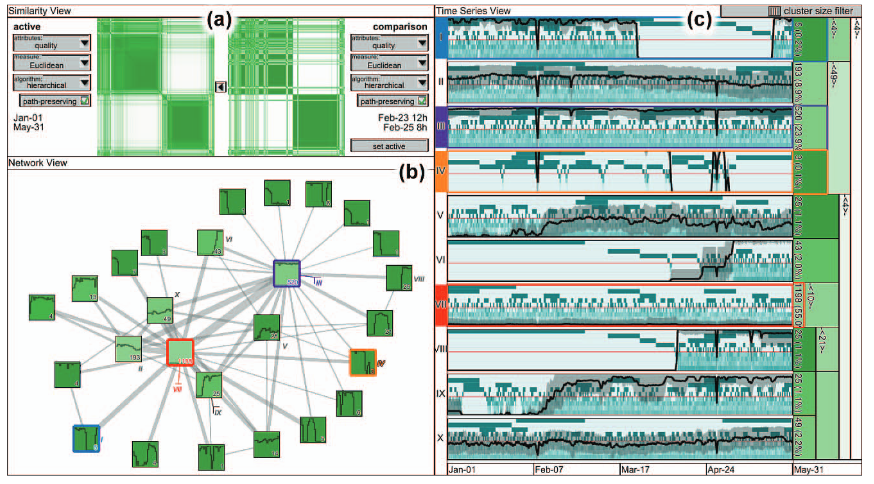
\includegraphics[trim={0 0 0 0}, width=140mm]{./Figures/hadlakClusteredTrends.png}
  \caption{The temporal trends are visualized in more detail in the time series view (c) by a multi-scale time plot for each visible cluster in the network view. The cluster hierarchy is shown on the right side of this view, also reflecting the intra-cluster similarity. Clusters (I, III, IV and VII ) selected for a closer inspection are highlighted in different colors in the network and time series view.\newline
  Figure and Caption taken from Hadlak et al. \cite{dynamicTrend}.}
  \label{fig:hadlakClusteredTrends}
  \end{center}
\end{figure}


\subsubsection*{The Vistorian - Nodelink}
The contributions in this report extend The Vistorian's nodelink diagram - another visualisation technique. When using a series of static nodelink diagrams there are two methods to visualise the changes - one after the other (time-multiplexed) or side by side (juxtaposed) \cite{vdnwmc}. The Vistorian's nodelink diagram uses a time-multiplexed method with a timeline to control which frames of time are shown. While The Vistorian's nodelink diagram is timeline based the novel approach taken in this report is measure based and visualised alongside the existing timeline based approach. Since the local measures values are calculated based on the time window set in the timeline and the global measures use it directly as an axis, the measure based approach is tightly intertwined with the timeline based approach. The measures themselves and their own accompanying visualisations are used to aid user's understanding of the networks changes - complementing the  timeline approach rather than replacing it.

\section{Measures}
Table \ref{Tab:Tcr} below summarises the measures that have been implemented. For the purposes of this report measures are defined as being either static or dynamic, and either local or global. A static measure quantifies some aspect of a static network and only takes into account one time frame when doing this - where a time frame is a unit of network change. Note that this could potentially be multiple changes in topology provided they all occur in the same instant. A dynamic measure on the other hand only makes sense in a dynamic context as it assumes more than one time frame - dynamic measures quantify an aspect of the network's change. A local measure is applied to each node, edge or attribute individually. In this report all local measures apply only to nodes. Global measures are applied to the network as a whole.

\begin{center}
\begin{table}[H]
\begin{tabular}{ |c|c|c|c| } 
\hline
 & Static & Dynamic \\
\hline
\multirow{3}{4em}{Local} & Degree Centrality & Local Volatility \\ 
& & Local Redundancy \\ 
& & Local Activation \\ 
\hline
\multirow{5}{4em}{Global} & Number of Connected Components & Global Volatility \\
 & Diameter & Global Activation \\
 & Density & Global Redundancy  \\
 & Number of Node Pairs &   \\
 & Number of Node Nodes &   \\
\hline
\end{tabular}
\captionof{table}{Measures Table\label{Tab:Tcr}}

\end{table}
\end{center}



\section{The Vistorian}
The Vistorian is a free, online, easy to use open source dynamic network visualisation tool which was designed primarily for historians. It provides four primary visualisations to investigate a network: matrix, dyanamic ego network, nodelink and geo-visualisation. This project will focus on the nodelink visualisation specifically, shown in Figure \ref{fig:vistorianOriginal}. 

\begin{figure}[h!]
  \begin{center}
  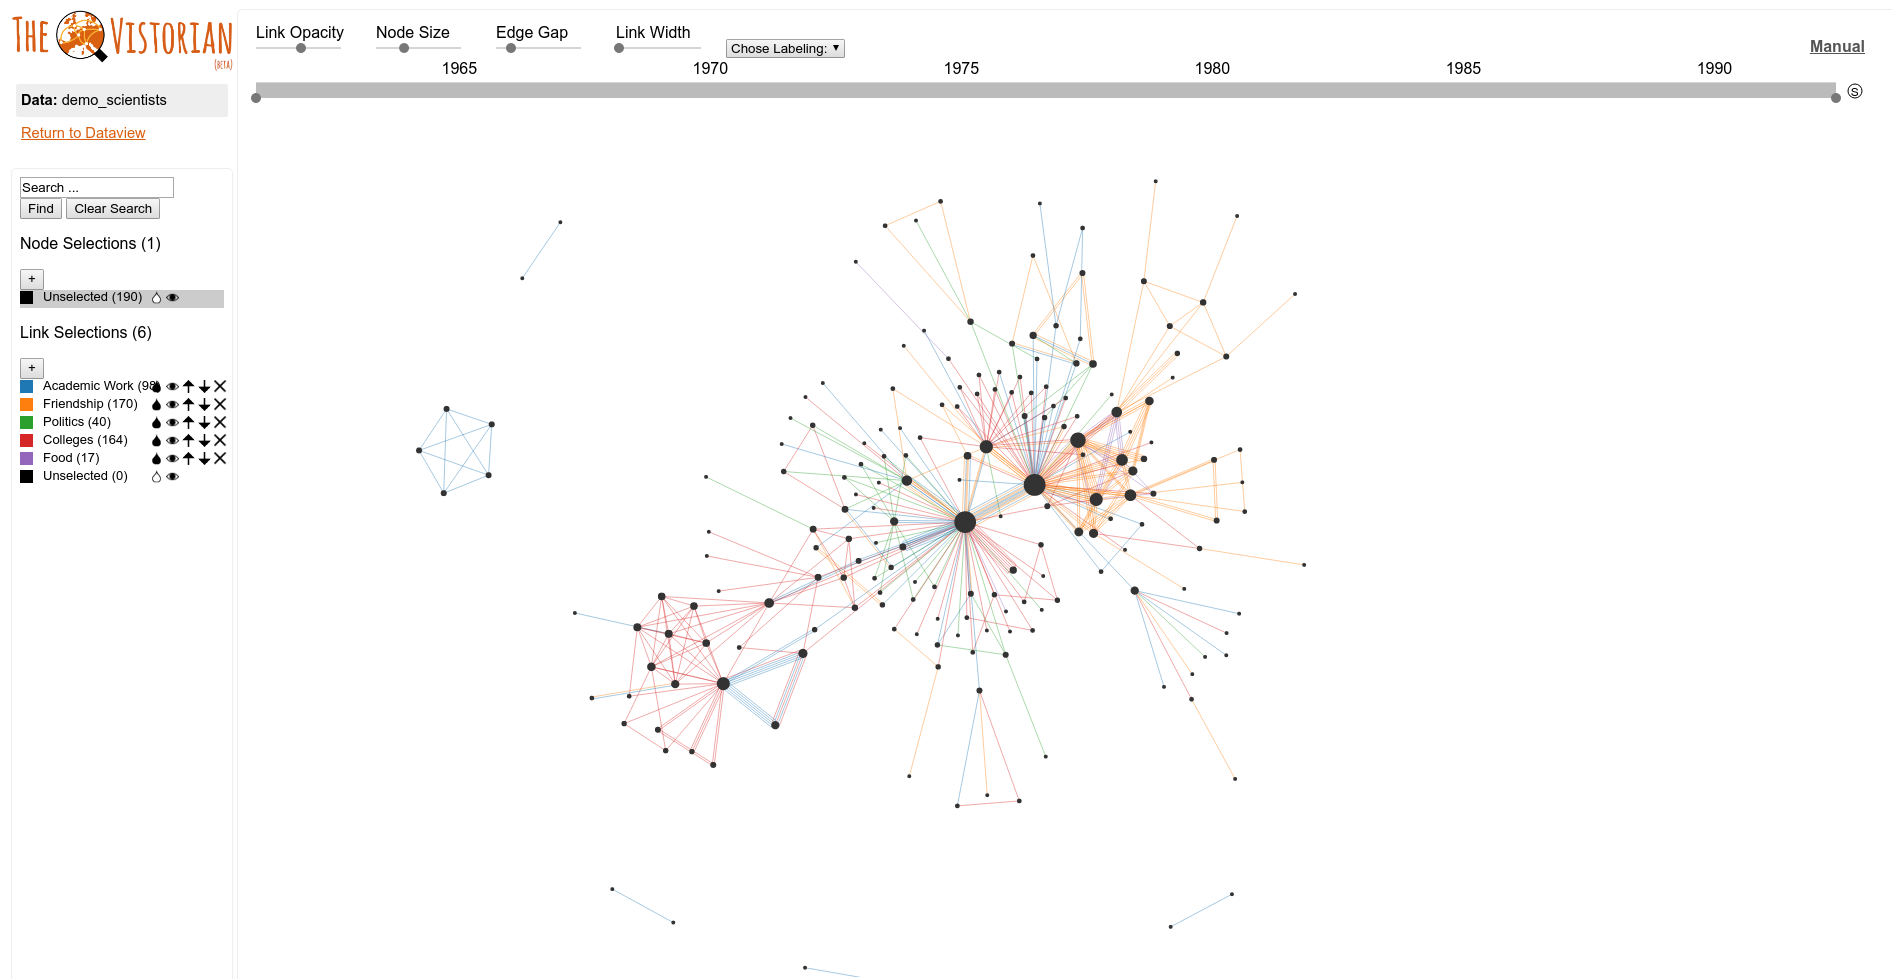
\includegraphics[trim={0 10cm 0 0}, width=140mm]{./Figures/vistorianOriginal.png}
  \caption{The Vistorian's Nodelink visualisation in it's original state.}
  \label{fig:vistorianOriginal}
  \end{center}
\end{figure}

The nodelink diagram is composed of nodes as points and edges as straight lines. The positions of nodes are kept the same during any change in the network topology, making it easier to visualise \cite{tsotaivg} and preserving the user's mental map\cite{tmitmmeridgd}. Coloured edges indicate different types of connection as specified in the network data.
%-Node-link history and development, why I'm using this one.\newline <-?
At the top of the network page is a time slider. Adjusting this time slider using the slider knobs filters the links shown if they are not present in that window. The slider can be moved left or right along the timeline, changing the selected period but maintaining the length of time. A force-directed layout is used, meaning that nodes with many common neighbours are drawn close to each other and nodes with fewer connections are moved to the edges. Node size is used to indicate the node degree and line colour indicates a specific type of relation. Edges are defined as the direct links between nodes and only exist during at most one time frame, whereas a nodepair is active if any edge is present between two nodes - meaning they can exist during multiple time frames provided there is at least one edge linking the nodes. In The Vistorian the network is split into discrete time frames where each time frame represents some change happening in the network.
More details are given in the visualization manual \cite{vismanual}

\subsubsection*{The codebase}
\label{sec:sec24}
The Vistorian was primarily written in TypeScript \cite{typescript} and D3 \cite{d3site}, a Javascript library. TypeScript is a typed superset of Javascript that compiles to Javascript. All of my additions were implemented using Javascript as I have more experience working with it directly. D3 was used for the visualisations because it provides an easy way to produce interactive visualisations in Javascript, and it was already in use within the Vistorian. 
As I was extending existing code, rather than starting from scratch there were some additional challenges. I had to learn how the existing systems operated to be able to properly extend and implement my own. Communication between iframes was particularly challenging - iframes are used to embed an html document within another document. The databar, bookmarks bar and network are all separate iframes. I built the databar as an iframe because it greatly increases flexibility as it means the window could be moved without affecting other components.


\subsubsection*{Summary}
GraphCuisine demonstrates that a network can be characterised by it's measures by generating a new network based on measure weights. In this report I invert this concept - using the measure weights to characterise an existing network - and adapt the concept to a dynamic context.
Hadlak et al. demonstrated that measures can be plotted over time to help visualise dynamic trends, however the graphs used in Figure \ref{fig:hadlakClusteredTrends} are overly complex and so a simpler and more intuitive approach was opted for instead.





